\chapter{Ausblick}
\label{ch:ausblick}
Dieses Kapitel soll einen Überblick über weitere größere Funktionen und Erweiterungen geben, durch die die Architektur,
die Webanwendung und die Smartphone-Apps erweitert und verbessert werden können.

Außerdem sollen Möglichkeiten aufgezeigt werden, welche die Arbeit mit Maschinen und Künstlicher Intelligenz
vereinfacht. Dazu zählt unter anderem eine Möglichkeit, eine direkte Verbindung zwischen Maschine und einem trainierten
Modell herzustellen.

Auch sind Themen, welche die klassische Container-Architektur verbessern für Erweiterungen interessant oder
Möglichkeiten zur schnelleren Vorhersage von Daten und der Eingabe von Daten unter erschwerten Bedingungen.

\section{Kontinuierliches Lernen und Optimieren}
Zu Anfang sollte eine Erweiterung aufgezeigt werden, welche die Möglichkeit bietet eine Maschine direkt mit einem
neuronalen Netz und einem trainierten Modell zu verbinden, um die Maschine schneller und ohne menschlichen Einfluss
einzustellen.

In der aktuellen Version der Architektur werden neuronale Netze auf der Basis von historischen Daten aufgebaut. Die so
trainierten Modelle werden in einem Deployment zur Verfügung gestellt und können ab dann Vorhersagen bearbeiten.

Einfacher wäre es, wenn eine Maschine eine direkte Verbindung zu einem neuronalen Netz hätte und diesem kontinuierliches
aktuelle Werte übergibt, mit denen zum Beispiel die Geschwindigkeit ermittelt werden kann mit der die Maschine arbeitet
oder wie viele korrekt bearbeitet wurden -- also die bearbeiteten Produkte abzüglich dem fehlerhaften Ausschuss.

Dies wäre möglich, indem man die Maschine mit einem IoT-Gateway ausstattet, welches verschiedenste Messgrößen aus der
Maschine extrahiert und mittels MQTT an die IBM Cloud schickt. Diese Daten könnte man dann auswerten, zusammenfassen
und dem Machine Learning Service als Stream zur Verfügung stellen.

In einem Modeler Flow kann man diesen Stream dann aufgreifen und ein neues Modell kontinuierlich trainieren, sodass sich
das Modell immer neuen Gegebenheiten anpassen kann. Die Vorhersagen, die das trainierte Modell dann ausgibt, basieren
dann auf den immer neuen Maschinenparametern.

Die Cloudant-Datenbank dient als Zwischenspeicher für die immer neuen Maschinenparameter, damit diese auch für
zukünftige Auswertungen bereitstehen. Als IoT-Gateway könnte das Bsoch eigene \textit{Rexroth IoT Device} dienen.

Die \textit{Internet of Things Plattform} kümmert sich um die Verbindung zum IoT-Gateway und die Übertragung der Daten
von der Maschine auf die Cloudant Datenbank.

Die Abbildung~\ref{fig:ausblick_uebersicht} auf Seite~\pageref{fig:ausblick_uebersicht} zeigt eine Übersicht über eine
Möglichen Architektur zur automatisierten Einstellung von Maschinenparametern.

\begin{figure}[h]
    \centering
    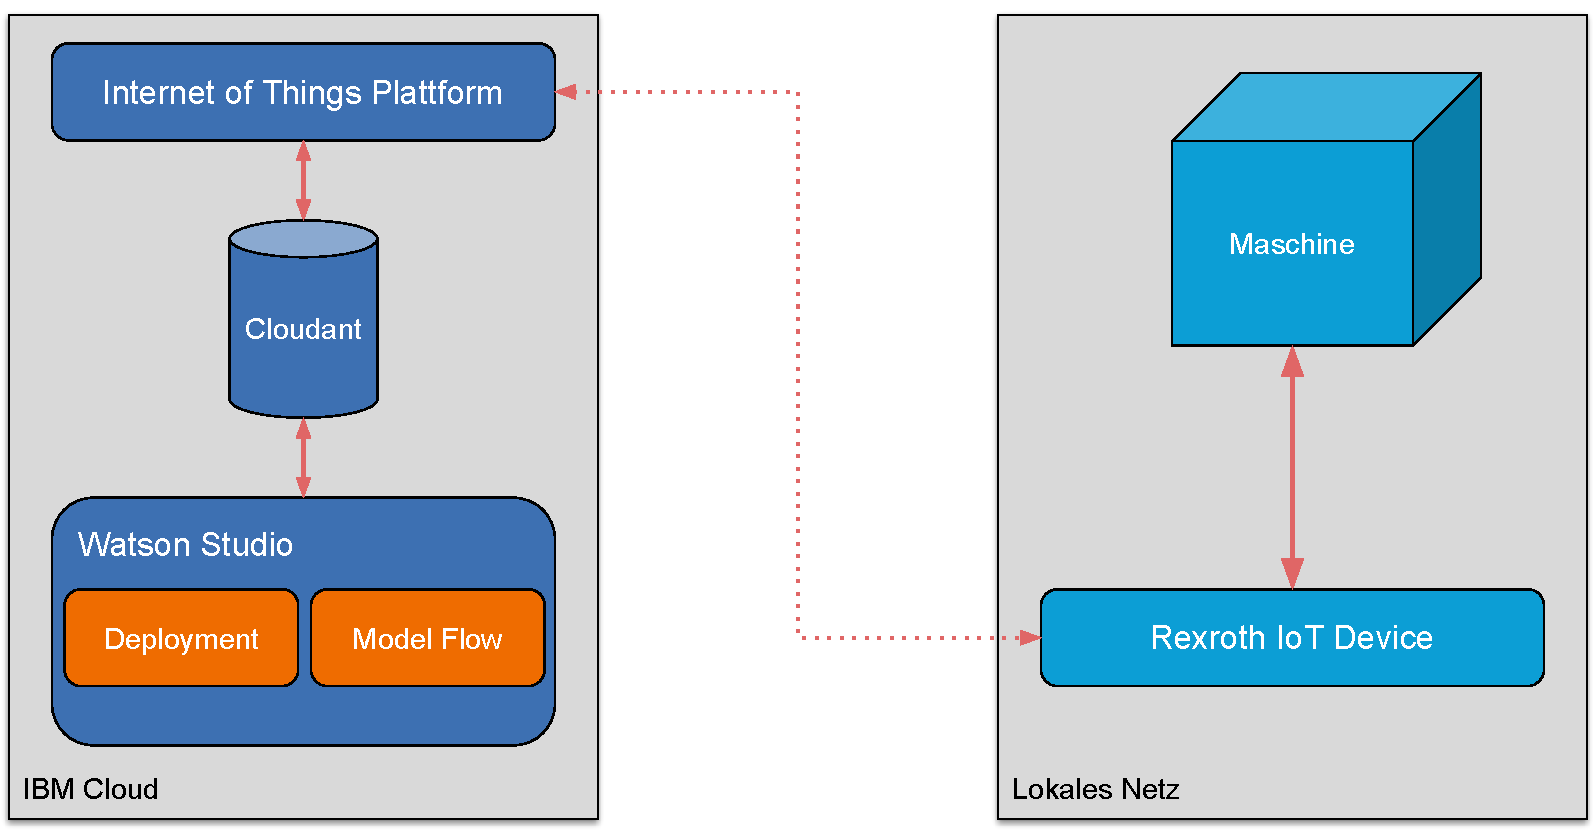
\includegraphics[width=\textwidth]{images/kapitel_6/architektur_uebersicht.pdf}
    \caption{Übersicht der Zielarchitektur}
    \label{fig:ausblick_uebersicht}
\end{figure}

Allerdings sind automatisierte Tests nicht immer und für jede Anwendung geeignet. Michael Lüttel von der Deutschen
Flugsicherung sagte auf der iqnite-Konferenz in Düsseldorf \enquote{Automatisierung macht nur dann Sinn, wenn sie mehr
Aufwände einspart als sie selbst erzeugt.}\footnote{https://www.qz-online.de/news/uebersicht/nachrichten/vor-und-nachteile-von-automatisierten-software-tests-890130.html}.

%% TODO noch schreiben
\section{Function as a Service}
Wie könnte man Functions/Lambda einbauen. FaaS

\colorbox{yellow}{Hier fehlt was}

%% TODO noch schreiben
\section{Machine Learning für Smartphones}
Wie könnte man das Feature nutzen und was würde das bringen

\colorbox{yellow}{Hier fehlt was}

%% TODO noch schreiben
\section{Offline Modus}
Ein Offline-Mode für die Website mit TensorFlow.js.

\colorbox{yellow}{Hier fehlt was}

%% TODO noch schreiben
\section{AI OpenScale}
\label{ai_openscale}
Hiermit kann man veranschaulichen, warum und wie die AI auf das Ergebnis gekommen ist. Das kann man mit dem Deployment
und mit dem TensorFlow.js Ding machen. Dafür braucht man eine Datenbank.

\colorbox{yellow}{Hier fehlt was}

%% TODO nosch schreiben
\section{Skalierbarkeit}
Wie könnte man die Anwendung skalieren?

\colorbox{yellow}{Hier fehlt was}

%% TODO noch schreiben
\section{Audit mit Blockchain}
Für die Waage muss Audit gemacht werden. Könnte man Blockchian da nicht noch einbauen?

\colorbox{yellow}{Hier fehlt was}

%% TODO noch schreiben
\section{Nutzen von IoT}
Nutzen von IoT

\colorbox{yellow}{Hier fehlt was}

\begin{figure}[h]
    \centering
    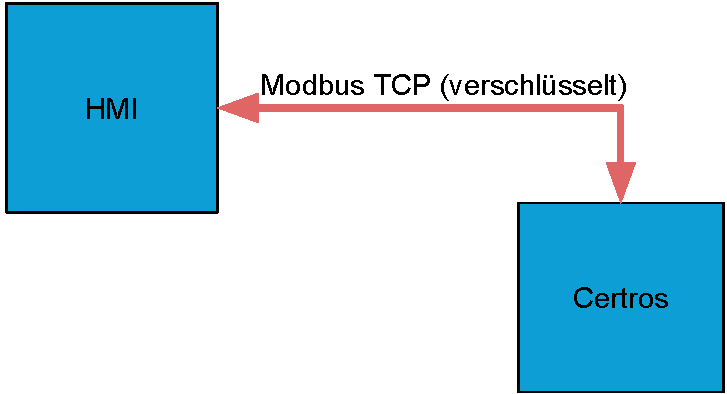
\includegraphics[width=\textwidth]{images/kapitel_6/iot_waage.pdf}
    \caption{Übersicht der Zielarchitektur}
    \label{fig:ausblick_iot}
\end{figure}

%% TODO noch schreiben
\subsection{Daten einlesen}
Wie könnten die Daten, welche durch das Netzwerk herausgefunden werden, auch automatisch in die Machine eingegeben werden?

\colorbox{yellow}{Hier fehlt was}

%% TODO noch schreiben
\subsection{Daten auslesen}
Wie könnte man Daten der Maschine auslesen, damit man sie nutzen kann um das Neuronale Netz weiter zu verbessern?

\colorbox{yellow}{Hier fehlt was}